
\documentclass[runningheads]{llncs}
\usepackage{graphicx}
\usepackage{apacite}
\usepackage{float}
\usepackage{listings}
\usepackage{float}
\usepackage[table]{xcolor}
\usepackage[toc,page]{appendix}
\usepackage{ucs}
\usepackage[utf8x]{inputenc}

\usepackage{hyperref}
\hypersetup{
	colorlinks=true,
	linkcolor=blue,
	filecolor=magenta,      
	urlcolor=cyan,
}

\usepackage[slovene]{babel}
\selectlanguage{slovene}

\lstset{
    breaklines=true,
    breakatwhitespace=true,
    inputencoding=utf8,
    extendedchars=false,
}

\renewcommand{\baselinestretch}{1.2} % za boljšo berljivost večji razmak
\renewcommand{\appendixpagename}{\normalfont\Large\bfseries{Appendix}}

\begin{document}

\title{Programming Assignment 2}
\subtitle{Implementing structured data extraction}

\author{
  Jaka Kokošar
  \and
  Danijel Maraž
  \and
  Toni Kocjan
}

\institute{Fakulteta za Računalništvo in Informatiko UL
\email{dm9929@student.uni-lj.si, jk0902@student.uni-lj.si, tk3152@student.uni-lj.si}\\
}

\maketitle             

\begin{abstract}
The article covers the work done in the scope of the second programming assignment as part of the subject web information extraction and retrieval. 

\keywords{Data Extraction Retrieval XPath Regex Roadrunner }
\end{abstract}

\section{Introduction}
After having collected the raw data with a crawler the logical next step is to convert it into a more structured format. As web pages do not have a strict shape this poses quite a challenge as any attempt of data extraction must be robust and resistant to various deformities in the html code. The report covers our attempts in implementing processes of structured data extraction in 6 different pages using basic methods such as regular expressions and xpath expressions. Alongside this an attempt was made to implement the RoadRunner algorithm which greatly simplifies the unpredictability aspect of data extraction.
\section{Description of chosen web pages and data items}
In addition to the mandatory websites, we selected a PZS\footnote{\url{https://www.pzs.si/}} ({\em Planinska zveza Slovenije}) site, which is the central register of information about the operation of mountain huts in Slovenia. As shown in Figure \ref{fig:Slika1}, we wanted to extract information of accommodations, location and contact details of a given hut. Since there are no other resources or APIs through which we could access this information and use them for any other purpose, we are forced to obtain information directly from this site.

\begin{figure}[H]
\begin{center}
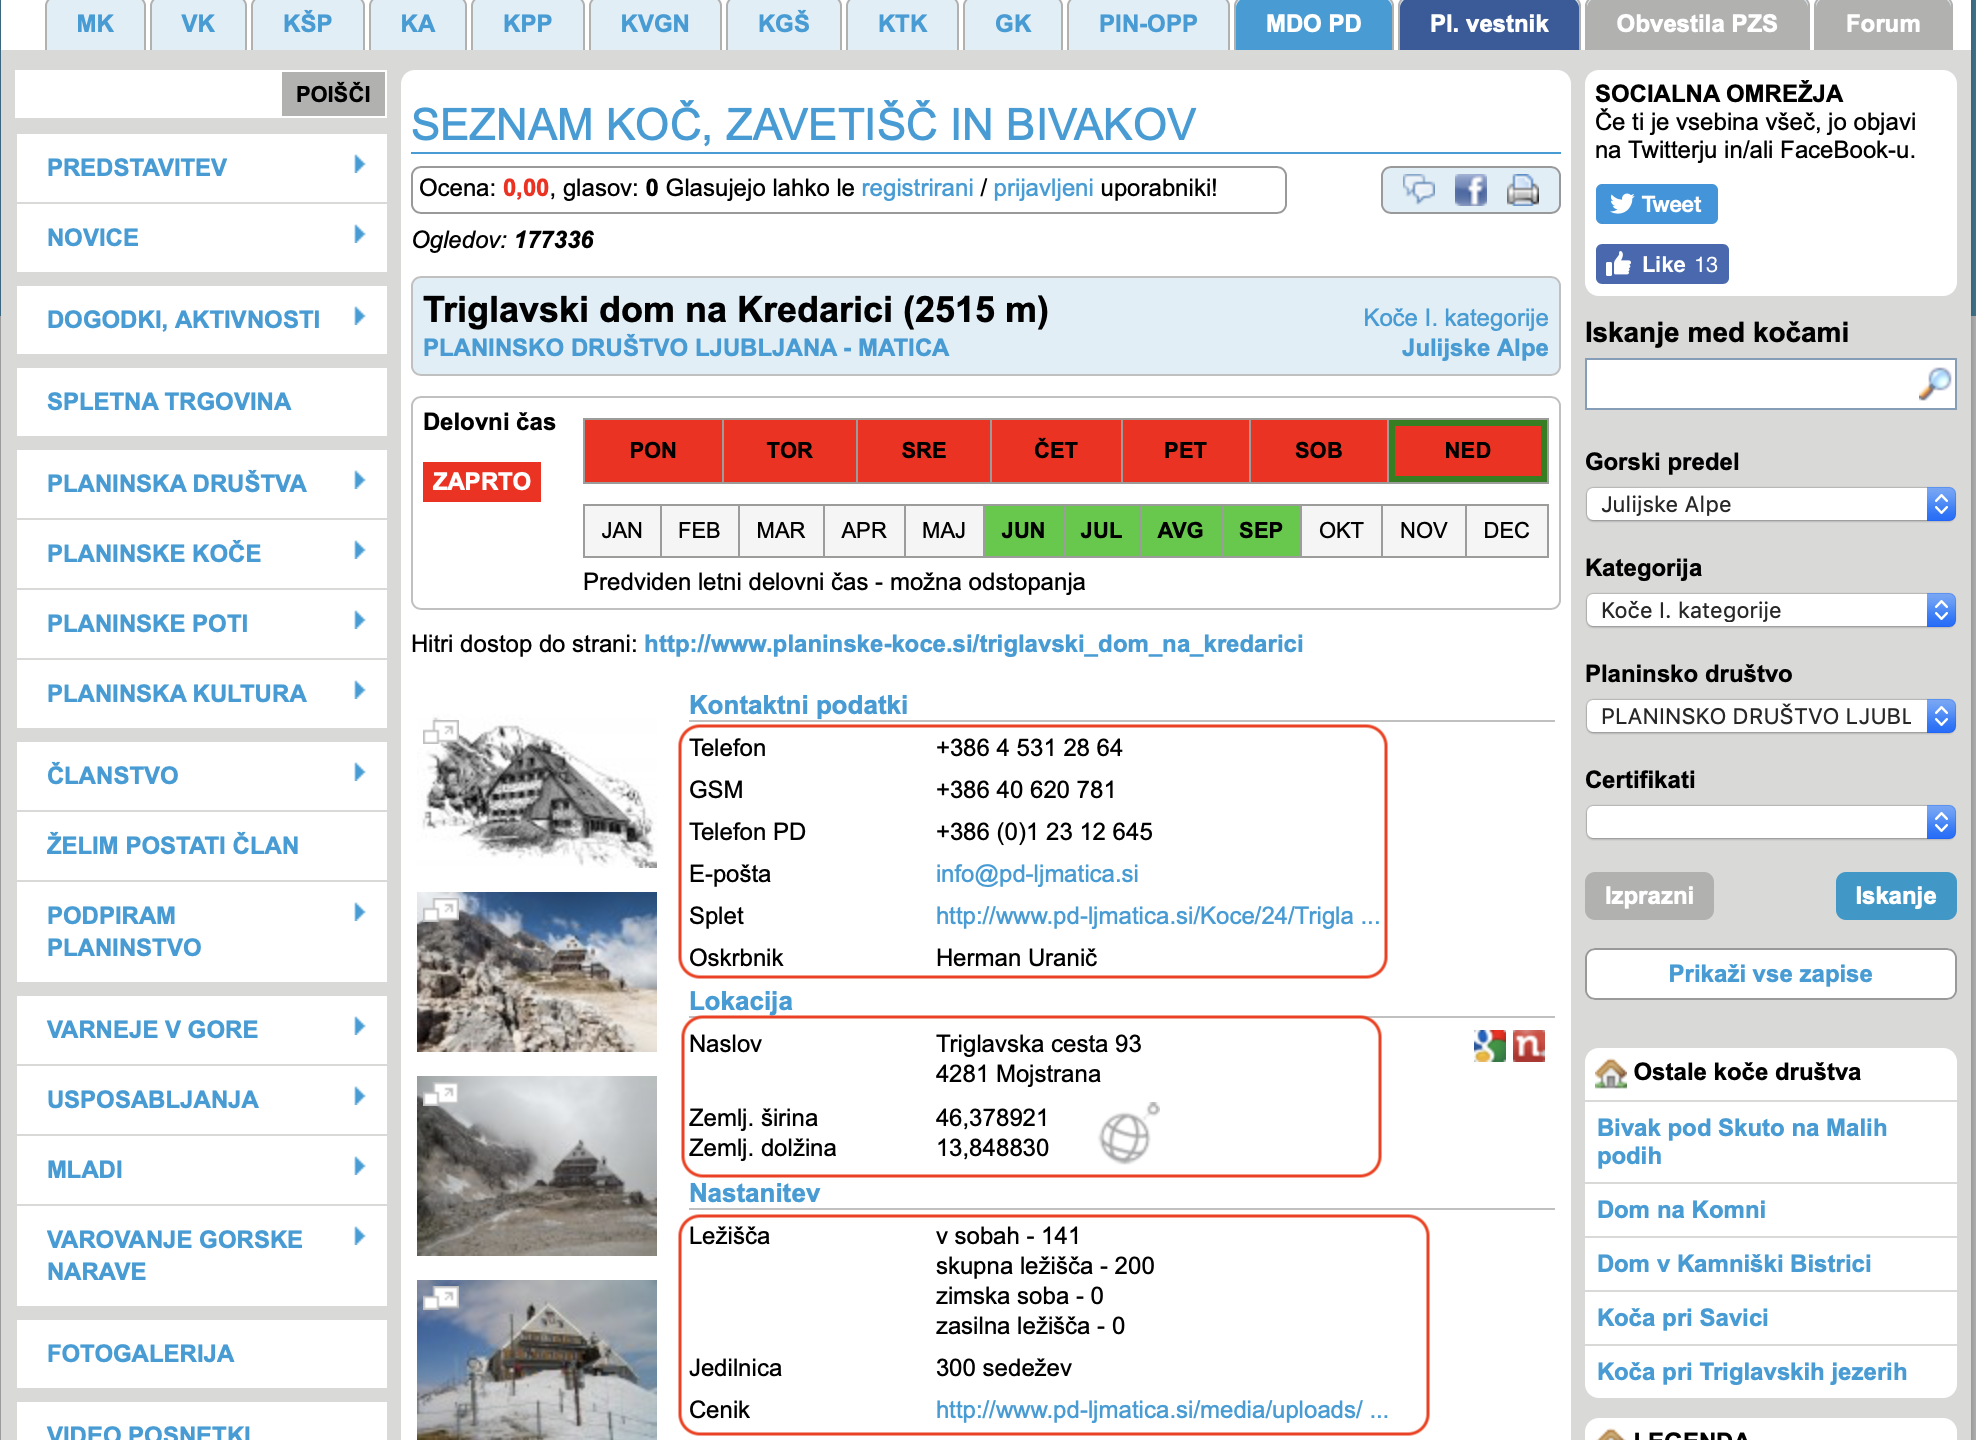
\includegraphics[scale=0.4]{pzs.png}
\caption{Data items we want to extract from pzs.si website}
\label{fig:Slika1}
\end{center}
\end{figure}

\section{Regular expressions implementation}
We defined three functions {\em parse\_rtv\_content},  {\em parse\_overstock\_content},  {\em parse\_pzs\_content}. Every function is responsible for a different page type but they are structured similarly. We extract data in three steps:
\begin{enumerate}
   \item read the input file
   \item pattern matching
   \item clean the results
\end{enumerate}
We only define one regular expression per page type. We extract all of the data items with a single expression in which we define all of the desired groups. After we obtain the results we clean the data of leftover html tags and strip newlines, whitespaces and tabulators. Results are available in the project repository\footnote{\url{https://github.com/LampDM/structured\_data\_extraction\_methods/tree/master/output/regex}}.

\section{XPath implementation}

\subsection{jewelry}
An initial Xpath expression is called on the input html which selects a \textit{tbody} element. The children of this element represent our jewelry and other items on the page. We count the number of children and with a for loop and extra Xpath expression access each data item that interests us for each child. Any children that are malformed or do not contain the items we're interested in (such as price etc.) encounter an exception as the Xpath expression throws an error and are automatically not processed. Afterwards some minor post-processing of the acquired strings is done and the json is created.
\subsubsection{Output}

\subsection{Cars}
The items Title, SubTitle, Author, PublishedTime and Lead are all collected via seperate XPath expressions on the input html as both pages have the same structure when it comes to them. The main difference between the two pages is the structure of the article body from which we've derived our Content item. We handle this by first extracting an article body tag which contains all the contents we need. Afterwards we give the extracted element as an argument to our function \textit{intr} which recursively iterates through the tag structure and appends all encountered text into a \textit{nonlocal} string. The string is then briefly processed and added to our json output.
\subsubsection{output1}
\subsubsection{output2}
\subsection{koce}
\subsubsection{output1}
\subsubsection{output2}

\section{RoadRunner like implementation}

RoadRunner algorithm is based on a technique called \textit{tree matching}, which automatically generates a common wrapper by exploiting similarities and differences among pages of same class. In principal it works as follow:
at every step, matching is performed on two objects: an input page and a reference page. [1]

\subsection{Implementation details}

We separate our algorithm into two stages:
\begin{itemize}
	\item tree parsing
	\item automatic wrapper generation
\end{itemize}

\subsubsection{Tree parsing}

The result of this stage is a tree-like representation of the HTML document. Each node in the tree contains information about a specific tag in the document, for instance tag's name, it's content, attributes and also it's children nodes. 

Parsing is divided into two sub-stages called \textit{Lexer} and \textit{Parser}:

Lexer produces a stream of tokens where each token represents and groups a meaningful subsequnce of characters from the source document (open tag, close tag, identifier, string literal, ...). 

Parser consumes stream provided by the lexer and builds the tree. Building process itself is quite straightforward since html does not contain many syntax rules. Altough the main problem of course is that HTML is not strict and that the documents being parsed can contain \textit{incorrect} sequence of tokens and still be successfuly rendered by the browser. For that purpose \textit{Parser} contains a simple error-recovery mechanism.

\subsubsection{Wrapper generation}

Wrapper is also a tree-like structure in which each node represents a result of a matching between a node from input page and a node from reference page. 

The algorithm \textit{preorderly} traverses both trees and compares current root nodes. If the nodes match in both tag name and content, they are marked as \textit{matching}. If instead they only match in tag name we also consider them matching, but they are marked as \textit{name-matching}. If they don't match at all we mark them as \textit{non-matching}.

We then recursively compare their children. A problem arises when nodes don't have the same number of children. There are several ways we can solve this problem: a simple solution is to just \textit{zip} both lists together and perform matching. A better solution might be to perform matching multiple times, each time moving the aligment of the smaller list by one, and select a matching with the least miss-matches.

\subsection{Results}

Results for all pages can be found inside the \textit{output/RoadRunner} directory.

More details can be found on our \href{https://github.com/LampDM/structured_data_extraction_methods/tree/master/RoadRunner}{Github}.

\href{https://www.researchgate.net/publication/221213613_RoadRunner_Automatic_data_extraction_from_data-intensive_Web_sites}{[1] Automatic data extraction}

\end{document}
